\newpage
\part{CRISP-DM Process Model}
The knowledge discovery process follows the following diagram: \textbf{Data Understanding -- Data Preparation -- Modeling -- Evaluation}. 
\begin{figure}[H]
	\centering
	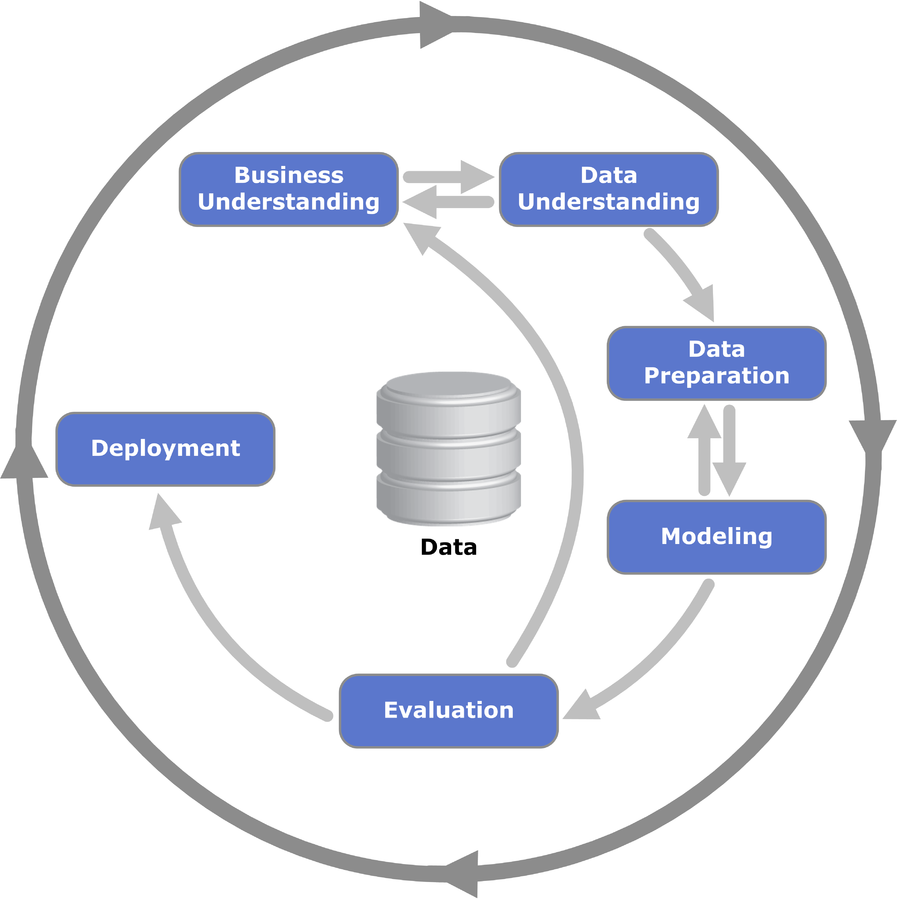
\includegraphics[width=0.45\textwidth]{CRISP-DM.png}
\end{figure}
\section{Data Understanding}
\subsection{Qualitative \& Quantitative Understanding}
Given a dataset description or an attribute table, 
\begin{itemize}
	\item Qualitative understanding:
	\begin{itemize}
		\item format of the data: \textbf{tidy data}?
		\item dependent \& independent variables
		\item scale of measurement of attributes: nominal/ordinal/interval/ratio
		\item cross-sectional, time-series, panel data?
	\end{itemize}
	\item Quantitative understanding
	\begin{itemize}
		\item \# instances, ideal: > 5000
		\item \# attributes, ideal start: < 50
		\item \# targets (balance of classes), ideal: > 100 each class
	\end{itemize}
\end{itemize} 
Ways to obtain understanding:
\begin{itemize}
	\item Visualization: histogram, distribution, relationship between attribute and response
	\item Summary: mean, median, attribute relationships
\end{itemize}

\subsection{Format of Data: tidy?}
\paragraph{Tidy Data} tabular data is tidy if
\begin{itemize}
	\item each \textbf{variable/feature} is in \textbf{single column}
	\item each \textbf{observation/instance} is in \textbf{single row}
	\item each \textbf{value} is in \textbf{single cell}.
\end{itemize}
\begin{figure}[H]
	\centering
	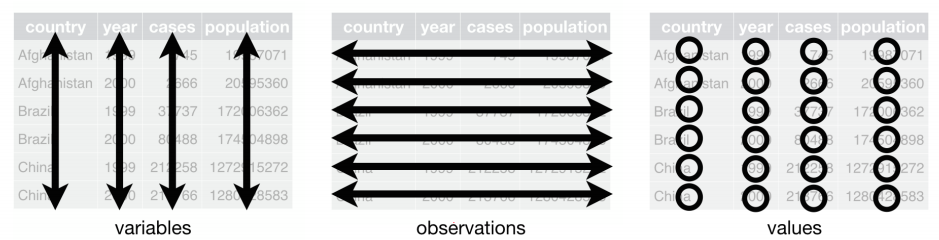
\includegraphics[width=\textwidth]{tidy.png}
\end{figure}
example of tidy data:
\begin{figure}[H]
	\centering
	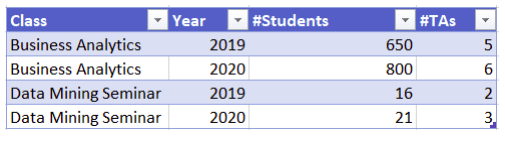
\includegraphics[width=0.6\textwidth]{tidy1.png}
\end{figure}
\paragraph{Wide Data} \textbf{same variable} is spanned into \textbf{multiple columns}. eg: year.
\begin{figure}[H]
	\centering
	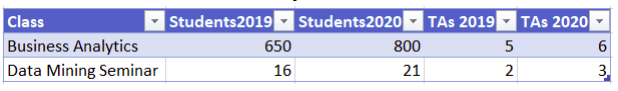
\includegraphics[width=0.7\textwidth]{wide.png}
\end{figure}
\paragraph{Long Data} \textbf{multiple variables} is compressed into \textbf{one column}. eg: n\_Students \& n\_TAs.
\begin{figure}[H]
	\centering
	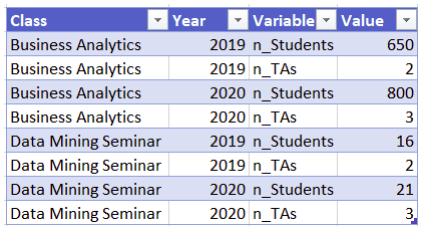
\includegraphics[width=0.5\textwidth]{long.png}
\end{figure}

\section{Data Preparation}
According to the data understanding, we distribute the data preparation also into these 3 parts.

But first of all, \textbf{tidy} the data if the format is long/wide. $\rightarrow$ pivoting.

The data preparation works on tidy data.
\subsection{Instance: Missing Value?}
Missing values need to be \textbf{standardized}:
\begin{itemize}
	\item \textbf{ignore} instance with missing values
	\item treat missing values as \textbf{separate value}
	\item \textbf{imputation}: mean/median
\end{itemize}
\subsection{Attributes: Conversion, Discretization \& Feature Selection}
\subsubsection{Conversion}
\begin{itemize}
	\item ordinal $\rightarrow$ numbers, preserving \textbf{natural order}.
	\item nominal 
	\begin{itemize}
		\item \#attribute values is small: nominal $\rightarrow$ numeric, \textbf{each attribute value} becomes a single \textbf{binary attribute} (number of binary classes: \textbf{(\#attributevalues - 1)} per attribute).
		\item \#attribute values is large: ignore (eg: IDs)
	\end{itemize}
	\item continuous numeric: Discretization, only if model requires(eg: naive Bayes).
\end{itemize}

\subsubsection{Discretization / Binning}
\begin{itemize}
	\item Reasons for Discretization:
	\begin{itemize}
		\item data: numeric data not normally distributed, data requires sorting frequently(decision tree).
		\item model: model requires nominal data as input(naive Bayes).
	\end{itemize}
	\item Reasons against Discretization:
	\begin{itemize}
		\item in decision tree: equi-depth bins \textbf{doesn't maximize the information gain}. Through the algorithm(binary split) we can find better splits instead of binning.
		\item will potentially \textbf{lose ordinal information}.
		\item model-dependent: regression models requires numeric data, no discretization.
	\end{itemize}
	\item Ways of Discretization:
	\begin{itemize}
		\item equi-frequency/depth
		\item class dependent: when decision tree classifier is used, \textbf{best split} according to \textbf{information gain}.
		\item order-preserving: numeric $\rightarrow$ k nominal $\rightarrow$ $(k-1)$ binary attributes, explaining comparison between $(i-1)$ and $i$.
	\end{itemize}
\end{itemize}
\subsubsection{Feature Selection}
\begin{itemize}
	\item Goal: choose the \textbf{most relevant subset}.
	\item Methods:
	\begin{itemize}
		\item Best Subset (search all, select best)
		\item Forward Selection (bottom-up)
		\item Backward Elimination (top-down)
		\item Stepwise Regression (combines forward/backward)
	\end{itemize}
	\item Use-Case: linear regression, classification, dimensionality reduction, regularization
	\item Ideal: at most 50.
\end{itemize}
\subsection{Targets: Balanced Train \& Test Set}
According to the distribution of targets, build up \textbf{balanced set} and then split into \textbf{balanced train set} and \textbf{balanced test set}. 
\begin{itemize}
	\item targets are balanced: each set gets \textbf{same amount} of targets
	\item targets are \textbf{unbalanced}: split \textbf{proportionally}.
\end{itemize}
This only applies to training \& fitting models. It doesn't apply to statistical inference.

